\documentclass[times,review,preprint,authoryear]{elsarticle}
%%\documentclass[times,final]{elsarticle}

\usepackage{jcomp}
\usepackage{framed,multirow}
\usepackage{amsmath,amsfonts,amssymb,amsthm}
\usepackage{latexsym}
\usepackage{url}
\usepackage{xcolor}
\usepackage{hyperref}
\usepackage{cleveref}
\usepackage{booktabs}
\usepackage{subfig}

\newtheorem{theorem}{Theorem}
\newtheorem{lemma}{Lemma}
\newtheorem{corollary}{Corollary}
\newtheorem{remark}{Remark}

\newcommand{\Rnum}{\mathbb{R}}
\newcommand{\Cnum}{\mathbb{C}}
\newcommand{\Znum}{\mathbb{Z}}
\newcommand{\Nnum}{\mathbb{N}}
\newcommand{\bx}{\mathbf{x}}
\newcommand{\by}{\mathbf{y}}
\newcommand{\bn}{\mathbf{n}}

\journal{Journal of Computational Physics}

\begin{document}

%\verso{Given-name Surname \textit{etal}}

\begin{frontmatter}

\title{A family of edge centered finite volume schemes for heterogeneous and anisotropic diffusion problems on unstructured meshes}

\author[1]{Ziqi \snm{Liu}\corref{cor1}}
\ead{liu-zq21@mails.tsinghua.edu.cn}

\author[2]{Shuai \snm{Miao}}
\ead{miaoshuai18@gscaep.ac.cn}

\cortext[cor1]{Corresponding author.}
\address[1]{Department of Mathematical Sciences, Tsinghua University, Beijing 100084, PR China}
\address[2]{Graduate School of China Academy of Engineering Physics,  Beijing, 100088, PR China}

\received{***}
\finalform{***}
\accepted{***}
\availableonline{***}
\communicated{***}

\begin{abstract}
This paper introduces a family of edge centered finite volume schemes for the stationary diffusion problems on general unstructured polygonal meshes. These schemes are locally conservative with respect to the dual mesh and have only edge centered unknowns with no extra auxiliary variable.
In this paper, we propose a general form of edge centered finite volume scheme basing on the linear preserving criterion and construct two particular schemes (EBS-1 and EBS-2). The EBS-2 leads to a symmetric positive definite matrix whose coercivity and convergence is rigorously analyzed.
Also, the relationship between edge centered schemes and the finite volume element method with Crouzeix-Raviart element and the finite difference method with X-shaped stencil is discussed.
Numerical experiments indicate that edge centered schemes have optimal convergence rates and are more robust than the existing cell centered scheme in some extreme cases.
\end{abstract}

% \begin{keyword}
% \MSC 41A05\sep 41A10\sep 65D05\sep 65D17
% \KWD locally conservative \sep finite volume scheme \sep diffusion equation \sep edge centered
% \end{keyword}

\end{frontmatter}

\section{Introduction}\label{sec1}

Anisotropic and heterogeneous diffusion problems arise in a wide range of scientific fields, such as Navier-Stokes equations \cite{???}, radiation hydrodynamics \cite{???}, petroleum reservoir simulation \cite{???}, and so on.
Severly discontinous solutions, highly distorted meshes and strongly anisotropic diffusion tensors make the problem difficult. It is hard to design an accurate and effective numerical scheme. Firstly, the regularity of the solution limits higher-order methods solving the problem. Secondly, to obtain a physical solution, the scheme should be locally conservative. Finally, the diffusion tensor is possibly anisotropic, which means that its eigenvalue may be small.

% cite FCCV, ???
In simulating a complex physical system, for example, Navier-Stokes equations, diffusion equation is usually coupled with a momentum equation. If the conventional mesh and central difference are used to discretize the diffusion process, the discrete form of momentum equation may not be able to detect the unreasonable pressure field. In order to solve this, an effective method is to use staggered mesh technology. In staggered mesh technology, the velocity is deifned on the cell interface and the pressure is stored on the cell centers. Therefore, the control volume of the velocity and pressure will have a dislocation of half a grid step. This is one of the main reasons why we construct this scheme, that is, to construct a finite volume scheme at the edge of the mesh, so that the Unknowns at the edge of the mesh and the Unknowns at the center can be decoupled.






In recent decades, many authors have conducted extensive research on the development of effective FV schemes.
The two-point flux approximation (TPFA) scheme  is  widely used in petroleum engineering in the early stage. The  well-known multi-point flux approximation scheme (MPFA) \cite{Aavatsmark2002, Aavatsmark1998}  uses the edge  unknowns as  auxiliary ones. The edge unknowns, usually defined at the edge midpoints,  are  eliminated by solving a  local system. Follow up development includes MPFA-L \cite{Aavatsmark2008} and MPFA-G \cite{Agelas2010}, etc.    The harmonic averaging  point (HAP) is a special point on the edge and the related auxiliary unknown has a simple and elegant two-point interpolation formula. A cell-centered scheme using HAP as the auxiliary unknown was proposed in \cite{Agelas-Eymard2009}.
Then it was extended to the  3D case \cite{Eymard-Herbin2012}.  Some other linear and nonlinear cell-centered schemes based on HAP can be found in \cite{Lipnikov2012, wugaodai2012, sunwuzhang2013, Gao-Wu2013}.  However, it is possible for HAP to be located outside of the edge, which will cause a possible loss of accuracy and even lead to completely wrong results \cite{Terekhov2017, WZhang2020, Xie-Xu2021}. The  Hybrid Mimetic Mixed (HHM) schemes,  including the  hybrid finite volume (HFV) scheme \cite{Eymard2010}, the  mixed finite volume (MFV) scheme \cite{Droniou2006}, and the  mimetic finite difference (MFD) schemes \cite{Brezzi2005_1,Brezzi2005_2, Shashkov1995,Morel1998}, have both cell-centered unknowns and edge (or edge-flux) unknowns. The  DDFV schemes  \cite{Hermeline2000, Andreianov2007, su2018} have  cell-centered unknowns and vertex unknowns simultaneously. There exist also FV schemes that have only vertex unknowns \cite{Edwards-Zheng, Wu-Gao-Dai}. The second category  defines the auxiliary unknowns at cell vertices. Typical examples include the  nine-point scheme or the diamond scheme  \cite{li1980, Y-J-P, Wu-Dai-Gao-Yuan, gao-wu,C-C-L-C}. There are so many papers on the design of interpolation algorithms for the vertex unknowns, see, e.g., \cite{Y-J-P, gao-wu}. These algorithms are either difficult to extend to 3D cases or less accurate in discontinuous cases \cite{MiaoWu2022}.  In addition, theoretical analysis, especially the coercivity analysis of the nine-point scheme or diamond scheme, is very difficult, and the introduction of auxiliary unknowns makes the problem even more serious \cite{Y-J-P}.
Based on the original idea in \cite{Potier CL},  nonlinear positive preserving cell centered FV schemes were studied in \cite{Lipnikov2007, yuan2008}. In this case,  the vertex unknowns are even required to be interpolated as the convex combinations of  cell-centered unknowns, which is  more difficult than the design of positivity-preserving schemes itself.
In order to overcome this difficulty, some positive-preserving cell-centered schemes without interpolation constraints were suggested \cite{J. Wu-Z. Gao, Z. Gao-J. Wu, Schneider2017}, but this approach introduces a certain  truncation error that is not easy to analyze. For a more  comprehensive review of the finite volume schemes, the readers are referred to, e.g., \cite{Droniou2014, Schneider2018}.









In this paper, we construct a family of linear edge centered finite volume schemes for heterogeneous and anisotropic diffusion problems. The main features of schemes can be summarized as follows:
\begin{itemize}
\item They have only edge centered unknowns without extra auxiliary variable.
\item They allow arbitrary discontinuities and full diffusion tensors.
\item They works on the star-shaped polygonal meshes.
\item They have small stencils.
\item It has nearly second-order accuracy for $L^2$ error of the numerical solution.
\item The numerical experiments indicate that the new schemes are robustness and cost-efficient.
\end{itemize}

The rest of this paper is organized as follows. In \cref{sec2}, we introduced the governing equation of the diffusion problem, the construction of the dual mesh and some notations. In \cref{sec3}, we perpose a general form and construct two edge centered schemes (EBS-1 and EBS-2) basing on the linear preserving criterion. In \cref{sec4}, the coercivity and stability of the scheme are studied. Some special cases are also analysised in \cref{sec4}. Numerical results are given in \cref{sec5} to show the performance of new schemes on some challenging issues. Finally, the conclusions and future works are summarized in \cref{sec6}.

\section{Problem and notation}\label{sec2}

\subsection{stationary diffusion problems}\label{sec:prob}

We consider a stationary diffusion problem
\begin{equation}\label{eq:prob}
\left\{
\begin{aligned}
- \nabla \cdot (\Lambda \, \nabla u) = f & \quad \bx \in \Omega, \\
u = g & \quad \bx \in \partial \Omega.
\end{aligned}
\right.
\end{equation}
where $\Omega \subset \mathbb{R}^2$ is an open bounded polygonal domain with boundary $\partial \Omega$, $u(\bx)$ is the unknown function, $f(\bx)$ is the source term, $g(\bx)$ defined on $\partial \Omega$ is the boundary data. $\Lambda(\bx)$ is the diffusion tensor, here $\Lambda$ should be symmetric and there exits two positive number $\underline{\lambda}, \overline{\lambda}$ satisfies
\begin{equation*}
\underline{\lambda} \, \|\mathbf{v}\|^2 \leq \mathbf{v}^T \, \Lambda(\bx) \, \mathbf{v} \leq \overline{\lambda} \, \|\mathbf{v}\|^2, \quad \forall \mathbf{v} \in \mathbb{R}^2, \forall \bx \in \Omega.
\end{equation*}
In this problem, $\Lambda$ is piecewise Lipschitz-continuous but possibly discontinuous on $\Omega$, which will result in the loss of regularity of the unknown $u$. We can only get $u \in H^1(\Omega)$ and  $\Lambda \, \nabla u \in H^{\text{div}}(\Omega)$ and cannot obtain higher-order regularity.

\subsection{Prime and dual mesh}\label{sec:mesh}

The construction of the primary and dual meshes is slightly different from traditional meshes.
Consider a mesh $\mathcal{M}$ composed of a finite number of disjoint polygonal cells. With each cell in the mesh, we associate one point which is called cell center. We assume that each cell is star-shaped with respect to its center, which means that all lines connecting the its center and its vertex are contained by the cell. In this paper, we chose the centroid of the cell as its center.
Based on the prime mesh $\mathcal{M}$, the line connecting a cell center and its surrounding vertex is called the dual edge. Each edge in the prime mesh is surrounded by four dual edges connecting a cell center and a vertex. The area surrounded by these four lines is called the edge control volume. Edge control volumes are combined to form the dual mesh $\mathcal{M}^*$.
Vertexes of $\mathcal{M}^*$ are same as the prime mesh, edges of $\mathcal{M}^*$ are the dual edges and cells of $\mathcal{M}^*$ are edge control volumes. \cref{fig:stencil} shows the polygonal prime mesh $\mathcal{M}$ and the dual mesh $\mathcal{M}^*$ on a square domain.

Without misleading, a cell of $\mathcal{M}$ or the center of corresponding cell are all denoted by $K$, an edge of $\mathcal{M}$ or the midpoint of corresponding edge or the corresponding edge control volume are all denoted by $E$, a cell vertex is denoted by $P$, and the dual edge in $\mathcal{M}^*$ is denoted by $\sigma$.
The set of dual edges surrounding the edge control volume $E$ is denoted by $\sigma(E)$.
$\bn_{E, \sigma}$ denotes the unit outer normal on the line $\sigma$ of edge control volume $E$. If $\sigma$ is the common edge of $E_1$ and $E_2$, there holds $\bn_{E_1, \sigma} = -\bn_{E_2, \sigma}$. When not mentioned, $\bn_{\sigma}$ represents the normal vector with anti-clockwise direction.
For a certain polygon cell $K \in \mathcal{M}$ with $m_K$ edges, as shown in \cref{fig:stencil}, the nodes is numbered anti-clockwise as $P_1, P_2, \cdots, P_{m_K}$. We denote $P_{m_K+1} = P_{1}, P_{0} = P_{m_K}$. Edges in dual edges are numbered similarly. The edge $E_i$ connects $P_{i}$ and $P_{i+1}$ and the line $\sigma_i$ connects $K$ and $P_{i}$.
The coordinates of the vertex $P_i$ is denoted by $\bx_i = (x_i, y_i)^T$ and the coordinates of the edge $E$ and the the cell center $K$ is denoted by $\bx_{E}$ and $\bx_{K}$ respectively.

\begin{figure}[h]
\centering
% \subfloat[prime and dual mesh]{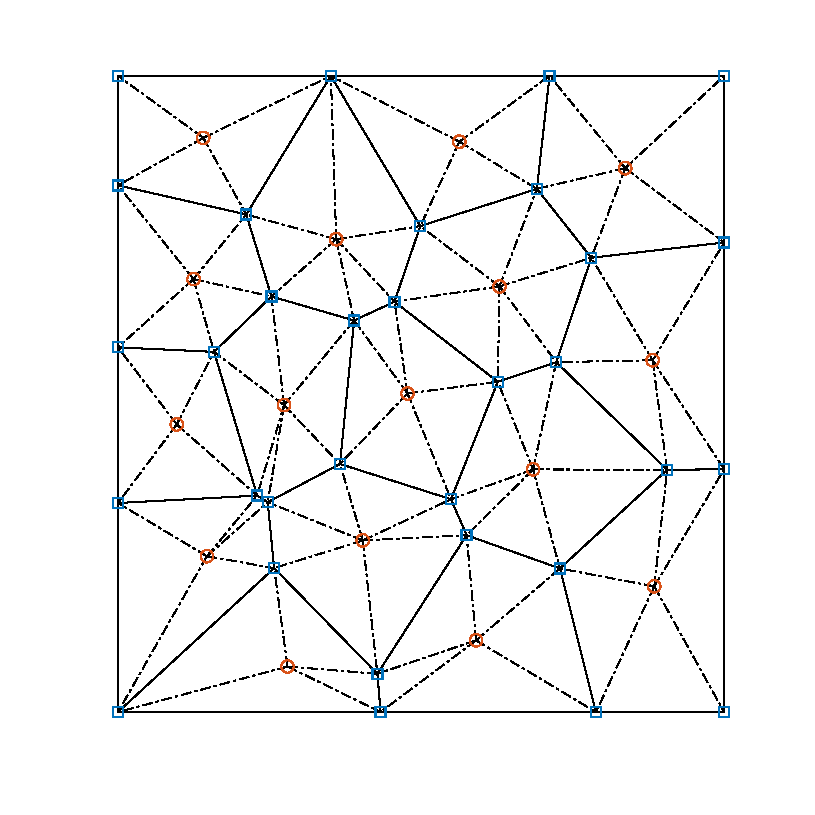
\includegraphics[width=0.5\linewidth]{pdm.eps}}\label{fig:mesh}
% \subfloat[notations and stencil]{\includegraphics[width=0.5\linewidth]{stencil.png} \label{fig:stencil}}
\caption{Notations and stencil}
\end{figure}

\section{Construction of the scheme}\label{sec3}

\subsection{A general form of edge centered finite volume scheme}

By integrating the problem \cref{eq:prob} over the edge control volume $E$, we obtain
\begin{equation}
- \int_{E} \nabla \cdot (\Lambda(x) \, \nabla u(x)) \ \mathrm{d}x = \sum_{\sigma \in \sigma(E)} \mathcal{F}_{E, \sigma} = \int_{E} f(x) \ \mathrm{d}x,
\end{equation}
where the continuous flux $\mathcal{F}_{E, \sigma}$ is
\begin{equation*}
\mathcal{F}_{E, \sigma} = - \int_{\sigma} (\Lambda(x) \, \nabla u(x)) \cdot \bn_{E, \sigma} \ \mathrm{d}x.
\end{equation*}
For two adjacent edge control volumes $E_1$ and $E_2$ with $\sigma$ as the adjacent edge, by continuity of the normal flux component, we have
\begin{equation*}
\mathcal{F}_{E_1, \sigma} = - \mathcal{F}_{E_2, \sigma}.
\end{equation*}

Next, we construct the flux approximations $F_{\sigma}$ on the dual edge $\sigma$ using the edge unknowns.
As shown in \cref{fig:stencil}, for a polygon $K$ in prime mesh, we put all flux on edges $\sigma_m$ into a vector and manipulate them together. In a linear scheme, all flux are approximated by a linear combination of the values of the solution on the middle points $E_m$. Considering that the formula should be exact for constant solutions, which means that the flux should be zero when the solution is constant. Then the flux is approximated by
\begin{equation}\label{eq:fluxapp}
\mathbf{F}_{K} = A_K \, \delta \mathbf{U}_{K},
\end{equation}
where $A_K$ is called cell matrix of size $m_K \times m_K$, and 
\begin{equation*}
\mathbf{F}_{K} = (F_{\sigma_m}, \ m = 1,2,\cdots,m_K)^T, \qquad \delta \mathbf{U}_{K} = (u(E_{m}) - u(E_{m-1}), \ m = 1,2,\cdots,m_K)^T
\end{equation*}
here, $\mathbf{F}_{K}$ is the vector of the flux approximations, and  $\delta \mathbf{U}_{K}$ is the vector of differences of edge unknowns.

Here, we establish the linearity-preserving criterion for the construction of the cell matrix $A_K$. The  linearity-preserving criterion means that a second order scheme should be exact for piecewise linear solutions whose diffusion is piecewise constant with respect to the primary mesh. By choosing the solution as $u(\bx) = x$ and $u(\bx) = y$, we can get the scheme satisfies the linear-preserving criterion if and only if
\begin{equation}\label{eq:lpmat}
N_{K} \, \Lambda_{K} = A_{K} \, X_{K},
\end{equation}
where
\begin{equation}\label{eq:defnx}
N_K = (- |\sigma| \, \bn_{\sigma_{m}}^T, \ m = 1,2,\cdots,m_K)^T, \qquad X_K = ((\bx_{E_{m}} - \bx_{E_{m-1}})^T, \ m = 1,2,\cdots,m_K).
\end{equation}
here $N_K$ and $X_K$ are two $m_K \times 2$ matrix, and $\Lambda_K$ is the constant approximation of the diffusion tensor on cell $K$. In this paper, $\Lambda_K$ is chosen as the value of $\Lambda(\bx)$ at the cell center.

The critical part of an edge centered scheme is constructing of the cell matrix $A_{K}$ such that the linearity-preserving criterion is fulfilled. Here we gave two construction following.

\subsection{Construction basing on vector decomposition}

For a linear solution and a constant diffusion tensor on a certain polygon $K$, for example, when we approximating the flux $\mathcal{F}_{E_{2}, \sigma_{2}}$, we have
\begin{equation}
F_{E_{2}, \sigma_{2}} = - \int_{\sigma_{2}} (\Lambda_K \, \nabla u) \cdot \bn_{E_{2}, \sigma_{2}} \ \mathrm{d}x = - |\sigma_{2}| \, (\Lambda_K^T \, \bn_{E_{2}, \sigma_{2}}) \cdot \nabla u.
\end{equation}
As shown in \cref{fig:stencil},we can decompose the vector $|\sigma_{2}| \, (\Lambda_K^T \, \bn_{E_{2}, \sigma_{2}})$ as the linear combination of vector $\overrightarrow{E_{2} E_{1}}$ and $\overrightarrow{E_{2} E_{3}}$, that is
\begin{equation}\label{eq:dcomp}
|\sigma_{2}| \, \Lambda_K^T \, \bn_{E_{2}, \sigma_{2}} = \alpha_{-} \, \overrightarrow{E_{2} E_{1}} + \alpha_{+} \, \overrightarrow{E_{2} E_{3}}.
\end{equation}
For a linear solution $u$, the gradient of $u$ along the direction  $\overrightarrow{E_{2} E_{1}}$ and $\overrightarrow{E_{2} E_{3}}$ can be written as
\begin{equation*}
\nabla u \cdot \overrightarrow{E_{2} E_{1}} = u(E_{1}) - u(E_{2}), \qquad \nabla u \cdot \overrightarrow{E_{2} E_{3}} = u(E_{3}) - u(E_{2}).
\end{equation*}
Then we can get the flux approximation for piece-wise linear solution
\begin{equation*}
F_{E_{2}, \sigma_{2}} = \alpha_{-} \, (u(E_{2}) - u(E_{1})) + \alpha_{+} \, (E_{2}) - u(E_{3})
\end{equation*}
where $\alpha_{-}, \alpha_{+}$ is given by vector decomposition \cref{eq:dcomp}.

For edge control volume $E_{1}$, we can get the flux approximation $F_{E_{1}, \sigma_{2}}$ similarly. Caution that the flux approximation $F_{E_{1}, \sigma_{2}}$ is represented by $u(E_{0}), u(E_{1}), u(E_{2})$, whose stencil is normally different from $F_{E_{2}, \sigma_{2}}$.

Now we have two flux approxiamations, in order to satisfy the local conservation law, we should combine them into one. Since that both flux approximation satisfy the linear preserving criterion, we take a simple average of the two approximations and get the final flux. Note that the direction $\bn_{\sigma_{2}} = \bn_{E_{1}, \sigma_{2}} = - \bn_{E_{2}, \sigma_{2}}$, the final flux writes
\begin{equation*}
F_{\sigma_{2}} = \frac12 (F_{E_{1}, \sigma_{2}} - F_{E_{2}, \sigma_{2}})
\end{equation*}
It is obvious that the final flux approxiamation satisfies the linear preserving criterion.

\subsection{Construction basing on matrix stabilization}

In this section, we firstly demonstrate the geometry relationship in polygnals.

\begin{lemma}[Shoelace Formula]\label{lemma:K}
Consider a polygon $K$ with $m_K$ edges, whose nodes $\bx_1 = (x_1, y_1), \bx_2 = (x_2, y_2), \cdots, \bx_{m_K} = (x_{m_K}, y_{m_K})$ is ranged anti-clockwise, then the area of $K$ is
\begin{equation}
|K| = \frac12 \sum_{m=1}^{m_K} (x_{m} \, y_{m+1} - x_{m+1} \, y_{m}).
\end{equation}
\end{lemma}

Then we can get the relationship between $N_K$ and $X_K$.

\begin{theorem}
For arbitrary polygon $K$, two matrices $N_K$ and $X_K$ are defined in \cref{eq:defnx}. Then we have
\begin{equation}
N_K^T \, X_K = |K| \, I_2,
\end{equation}
where $I_2$ represents the $2 \times 2$ identity matrix.
\end{theorem}

\emph{proof}

For a polygon $K$ with $m_K$ nodes $\bx_1, \bx_2, \cdots, \bx_M$ and center $\bx_K$, we have
\begin{equation*}
|\sigma_m| \bn_m = \mathcal{R} \, (\bx_m - \bx_K), \qquad
\bx_{E_m} - \bx_{E_{m+1}} = \frac12 \, (\bx_{m-1} - \bx_{m+1}), \qquad
\mathcal{R} = \left(\begin{matrix}
0 & 1 \\
-1 & 0 \\
\end{matrix}\right)
\end{equation*}
where $\mathcal{R}$ represents the rotation matrix.

Since the formula is translation invariant, we can shift the center of the polygon to zero. Then we have
\begin{equation*}
N_K^T \, X_K = \frac12 \sum_{m=1}^{m_K} \mathcal{R} \, (\bx_m - \bx_K) \, (\bx_{m-1} - \bx_{m+1})^T = \frac12 \sum_{m=1}^{m_K} \mathcal{R} \, \bx_m \, (\bx_{m-1} - \bx_{m+1})^T,
\end{equation*}
and then
\begin{equation*}
N_K^T \, X_K = \frac12 \sum_{m=1}^{m_K} \left(\begin{matrix}
y_{m} \, (x_{m-1} - x_{m+1}) & y_{m} \, (y_{m-1} - y_{m+1}) \\
x_{m} \, (x_{m+1} - x_{m-1}) & x_{m} \, (y_{m+1} - y_{m-1}) \\
\end{matrix}\right)
\end{equation*}

Using \cref{lemma:K}, we have
\begin{equation*}
|K| = \frac12 \sum_{m=1}^{m_K} y_{m} \, (x_{m-1} - x_{m+1}) = \frac12 \sum_{m=1}^{m_K} x_{m} \, (y_{m+1} - y_{m-1}),
\end{equation*}
and
\begin{equation*}
\sum_{m=1}^{m_K} x_{m} \, (x_{m-1} - x_{m+1}) = \sum_{m=1}^{m_K} y_{m} \, (y_{m+1} - y_{m-1}) = 0.
\end{equation*}

Finally we can get
\begin{equation*}
N_K^T \, X_K = \left(\begin{matrix}
|K| & 0 \\
0 & |K| \\
\end{matrix}\right)
= |K| \, I_2.
\end{equation*}

\begin{remark}
This theorem can be seen as a extension of the Lemma 3.1 in \cite{wu_vertex-centered_2016}. It is essential to construct a symmetric positive difine cell matrix.
\end{remark}

Multiplying \cref{eq:lpmat} with $\frac{1}{|K|} \, N_K^T$, and comparing both side, we can find that if we choose
\begin{equation*}
A_K = \frac{1}{|K|} \, N_K \, \Lambda_{K} \, N_K^T,
\end{equation*}
the linear preserving condition will be satisfied. Nevertheless, cell matrix $A_K$ of this form is symmetric but only semi-positive definite, which will be proofed later.

Motivated by \cite{dong_analysis_2020}, we add a stabilized term and get
\begin{equation*}
A_K = \frac{1}{|K|} \, N_K \, \Lambda_{K} \, N_K^T + \gamma_K \, C_K, \quad \text{with} \quad C_K = I_K - X_K \, (X_K^T \, X_K)^{-1} \, X_K^T,
\end{equation*}
where  $I_K$ is an $m_K \times m_K$ identity matrix, $\gamma_K$ is a positive called stabilization parameter. In our numerical experiments, by taking into account the accuracy and robustness, the parameter is chosen as $\gamma_K = 3$.

\section{Analysis of Edge-Centered Schemes}\label{sec4}

\subsection{Convergence analysis}

We have seen that cell matrix plays an important role in the new vertex-centered scheme, and different cell matrices will result in different schemes. In this section, we shall make use of the special structure of polygonal meshes to construct a symmetric and positive definite cell matrix such that the linearity-preserving criterion is satisfied.



% \begin{lemma}
% $X_k^T \, X_K$ is a 2 × 2 non-singular matrix, and $C_K$ forms the null-space of $X_K$.
% \end{lemma}

\begin{lemma}
$A_K$ is SPD, 
\end{lemma}

\begin{theorem}
covercity
\end{theorem}

\subsection{Two special cases of the scheme}

\subsubsection{Edge centered scheme on triangular mesh}

For triangular meshes, all edge centered schemes satisfying linear preserving criterion reduce to the finite volume element method with Crouzeix-Raviart element (CR-FVEM). Therefore, the result above can also serve as the mesh construction and the convergence analysis for CR-FVEM.

In CR-FVEM, the problem \cref{eq:prob} is firstly written into weak form
\begin{equation*}
\int_{\Omega} (\Lambda(x) \, \nabla u(x)) \cdot \nabla v(x) \ \mathrm{d}x = \int_{\Omega} f(x) \, v(x) \ \mathrm{d}x, \quad \forall v \in L^2(\Omega).
\end{equation*}
For a triangular mesh $\mathcal{T}_h$, we can define a dual mesh $\mathcal{T}^*_h$ using the process in \cref{sec:mesh}, then the trial and test function space is chosen as
\begin{equation*}
S_h = \{u \in L^2(\Omega): \; u|_{K} \ \text{is linear} \ \forall K \in K(\mathcal{T}_h), \ u \ \text{is continuous at} \ E \ \text{and} \ u|_{\partial \Omega}(E) = u_0(E) \ \forall E \in E(\mathcal{T}_h)\},
\end{equation*}
and
\begin{equation*}
S^*_h = \{v \in L^2(\Omega): \; v|_{E} \ \text{is constant} \ \forall E \in K(\mathcal{T}^*_h), \ v|_{\partial \Omega} = 0\}.
\end{equation*}
Since the test function is piecewise constant on the dual mesh, the numerical scheme comes to finding $u \in S_h$, such that
\begin{equation}\label{eq:crfvem}
- \int_{E} \nabla \cdot (\Lambda(x) \, \nabla u(x)) \ \mathrm{d}x = - \int_{\partial E} (\Lambda(x) \, \nabla u(x)) \cdot \bn \ \mathrm{d}x = \int_{E} f(x) \ \mathrm{d}x, \quad \forall E \in K(\mathcal{T}^*_h).
\end{equation}
When we compute \cref{eq:crfvem} by numerical integration, the function is approximated by piecewise constant $\Lambda(x) \approx \Lambda_K, K \in \mathcal{T}_h$. According to the linear-preserving property of edge centered schemes, the integration is computed exactly in the scheme. Then we can get that on triangular meshes, all edge centered schemes satisfying linear preserving criterion are same, and they will reduce to CR-FVEM.

\subsubsection{Edge based scheme on uniform mesh}

Consider problem \cref{eq:prob} with a constant scalar diffusion coefficient on the square domain $\Omega = [0,1]^2$. We will show that when solving the problem on a uniform mesh, the EBS-1 will reduce to the traditional five-point finite difference scheme with rotation.

% \begin{figure}[h]
% \centering
% \subfloat[stencil of FDM]{\includegraphics[width=0.3\linewidth]{pics/fdm.eps}}
% \subfloat[stencil of EBS-1]{\includegraphics[width=0.3\linewidth]{pics/ebs1.eps}}
% \caption{Stencils of the finite difference scheme and EBS-1 on the uniform mesh.}
% \label{fig:fdm}
% \end{figure}

Consider a uniform mesh with step size $h$, as shown in \cref{fig:fdm}, in the finite difference scheme, unknowns are defined on edges denoted by $u_{i,j+1/2}$ and $u_{i+1/2,j}$. Using the Talyor expansion and the symmetry, we can get a finite difference approximation writes
\begin{equation*}
\triangle u_{i,j+1/2} = \frac{2}{h^2} \, (u_{i+1/2,j+1} + u_{i+1/2,j} + u_{i-1/2,j+1} + u_{i-1/2,j} - 4 \, u_{i,j+1/2} ) + \mathcal{O}(h^2).
\end{equation*}
The derivation the approximation of $\triangle u_{i+1/2,j}$ is similar. Noting that $\Lambda$ is a constant scalar, then we can get a finite difference scheme
\begin{equation}\label{eq:fdm}
-\Lambda \, (u_{i+1/2,j+1} + u_{i+1/2,j} + u_{i-1/2,j+1} + u_{i-1/2,j} - 4 \, u_{i,j+1/2}) = \frac{h^2}{2} \, f_{i,j+1/2}.
\end{equation}
The scheme can be seen as the rotation of the traditional five-point finite difference method, whose monotonicity and stability have been demonstrated.

Now we consider the EBS-1 on the uniform mesh. As shown in \cref{fig:fdm}, in a certain cell $K$, we have $|\sigma| \bn = \overrightarrow{E_2 E_1}$. Then in the vector decomposition \cref{eq:dcomp}, we have $\alpha_1 = 1, \alpha_2 = 0$, and the numerical flux on $\sigma$ is $F_{E_1, \sigma} = -F_{E_2, \sigma} = \Lambda (u(E_1) - u(E_2))$. On the other hand, noting that the measurement of each edge control volume is $h^2$ in the uniform mesh, when we compute the integral of $f(x)$ on the edge control volume using numerical quadrature the integreal writes $\frac{h^2}{2} f(E)$. Finally, we can get that the EBS-1 on the uniform mesh is equal to the finite difference scheme above.

\section{Numerical experiments}\label{sec5}

Here, we provide some numerical tests to show the performances of edge centered schemes.The edge centered schemes are compared with a traditional cell-centered method MPFA \cite{???}.

The errors of the scheme are evaluated by the following mesh-dependent norms.
For solutions defined on edges or cells in mesh $M$, the mesh-dependent $L^2$ and $L^{\infty}$ norms are defined as following respectively:
\begin{equation}
\|U\|_{2} = \sqrt{ \sum_{\mathcal{A}} |\mathcal{A}| \, |U_{\mathcal{A}}|^2 }, \qquad \|U\|_{\infty} = \max_{\mathcal{A}} |U_{\mathcal{A}}|, 
\end{equation}
where $\mathcal{A}$ represents each edge or each cell in the mesh $M$ and $|\mathcal{A}|$ represents the measurment of the edge control volume or the cell respectively.
Then the $L^p \ (p = 2, \infty)$ relative error of the numerical solution $U$ are defined as following respectively:
\begin{equation}
E_{p} = \frac{\|U - U_{\text{exact}}\|_{p}}{\|U_{\text{exact}}\|_{p}},
\end{equation}
where $U_{\text{exact}}$ is the value of the exact solution at the midpoint of each edge or the center of each cell.
The rate of convergence $R_{p} \, (p = 2, \infty)$ is obtained by computing the following formula on each two successive meshes $M_1$ and $M_2$:
\begin{equation}
R_{p} = -2 \frac{\log E_{p}(M_1) - \log E_{p}(M_2)}{\log \text{DoF}(M_1) - \log \text{DoF}(M_2)},
\end{equation}
where $\text{DoF}(M)$ represents the number of unknowns in the scheme, which is equal to the number of edge of the mesh $M$ for edge centered schemes and the number of cell for cell centered schemes.

Following numerical examples are taken from the benchmark proposed at fifth conference on discretization schemes for anisotropic diffusion problems on general grids \cite{???}. For EBS-2, the stabilization parameter is chosen as $\gamma = 3$ if not mentioned.

\subsection{Linear preserving}

To verify the linear preserving property of the edge schemes, we consider a problem on $\Omega = [0,1]^2$ with identity diffusion coefficient and linear exact solution
\begin{align*}
\Lambda(x) =
\left(
\begin{matrix}
1 & 0 \\
0 & 1
\end{matrix}
\right),
\qquad
u(x,y) = x + y + 1.
\end{align*}
We conduct this test on the locally refined mesh, random polygonal mesh, skewed quadrilateral mesh, Kershaw mesh, triangular mesh and sin mesh. The meshes used in this test are shown in \cref{fig:mesh}. The results are presented in \cref{tab:linear}. Table shows that the error of both schemes on all tested meshes close to machine precision, which means that both scheme reproduce the exact solution.

\begin{figure}[h]
\centering
\subfloat[locally refined mesh]{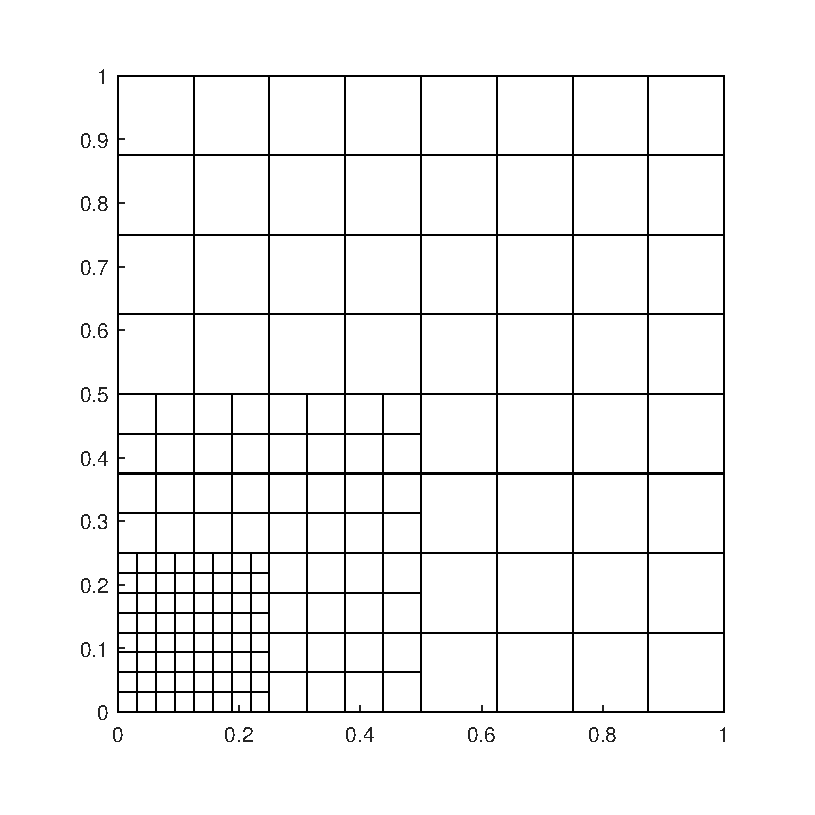
\includegraphics[width=0.3\linewidth]{pics/m1.eps}}
\subfloat[random polygonal mesh]{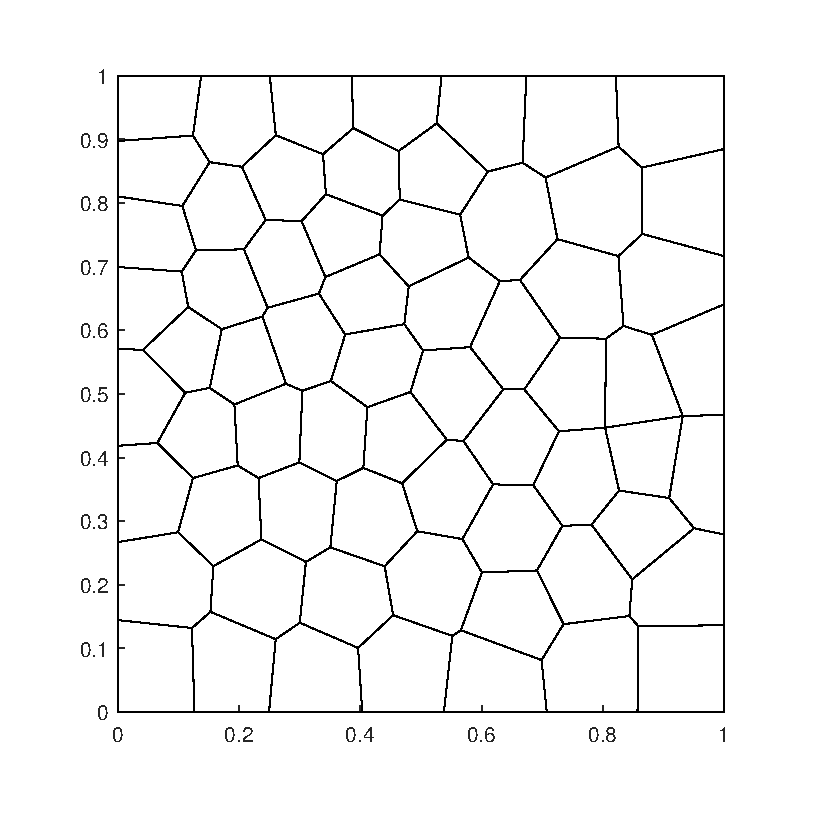
\includegraphics[width=0.3\linewidth]{pics/m2.eps}}
\subfloat[skewed quadrilateral mesh]{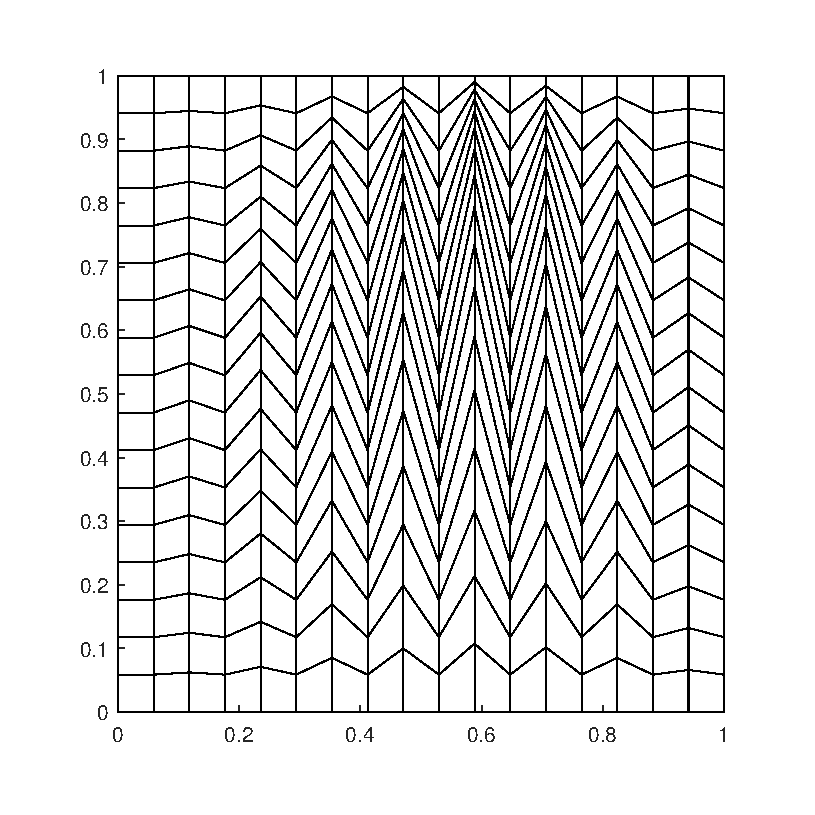
\includegraphics[width=0.3\linewidth]{pics/m3.eps}} \\
\subfloat[Kershaw mesh]{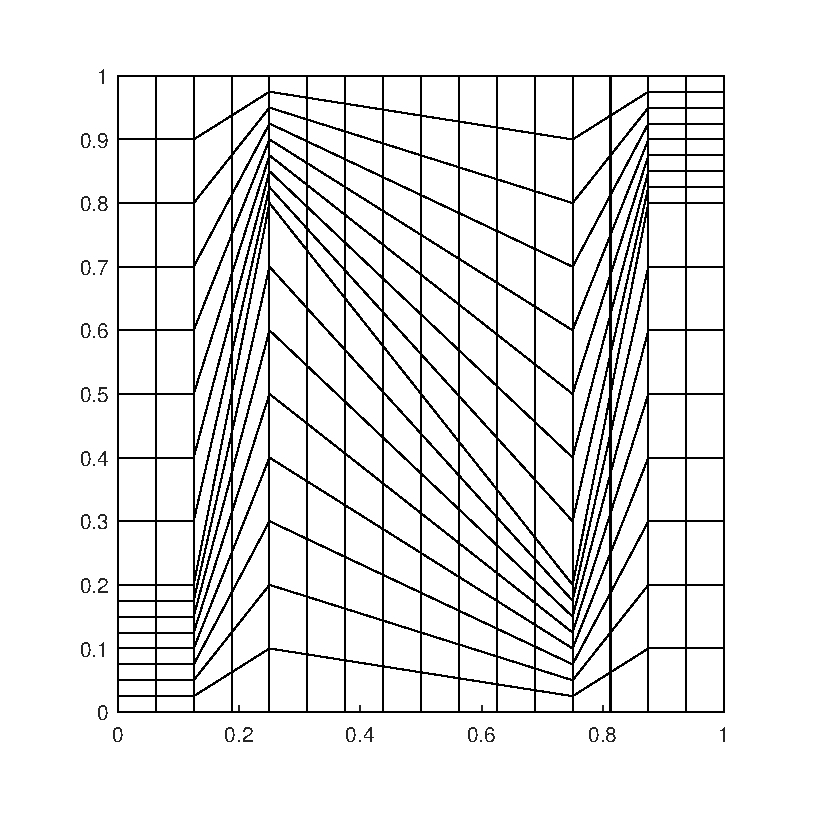
\includegraphics[width=0.3\linewidth]{pics/m4.eps}}
\subfloat[triangular mesh]{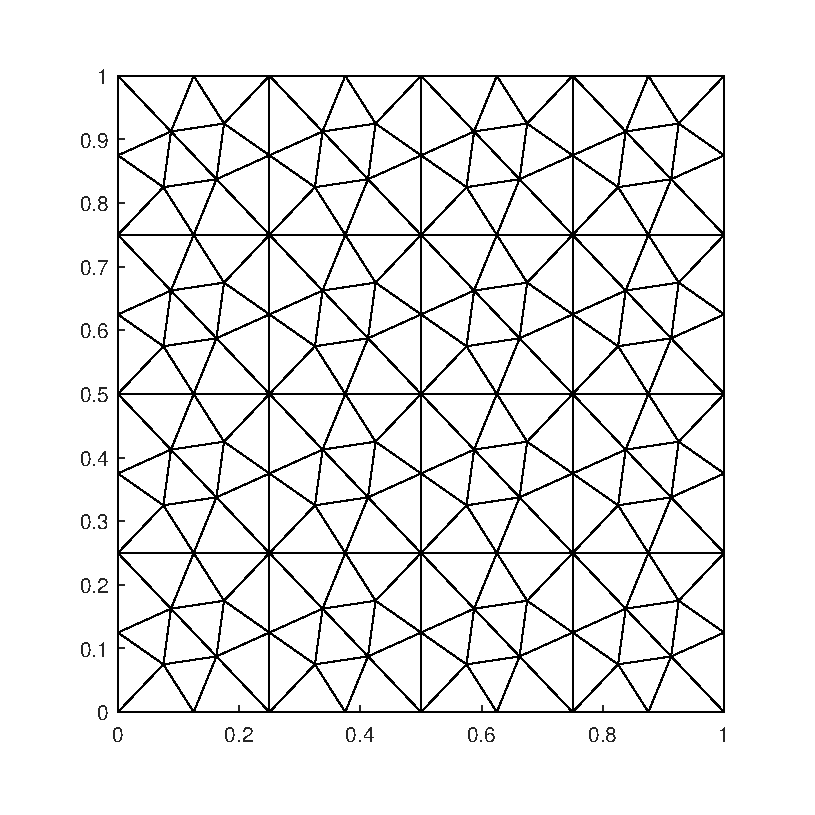
\includegraphics[width=0.3\linewidth]{pics/m5.eps}}
\subfloat[sin mesh]{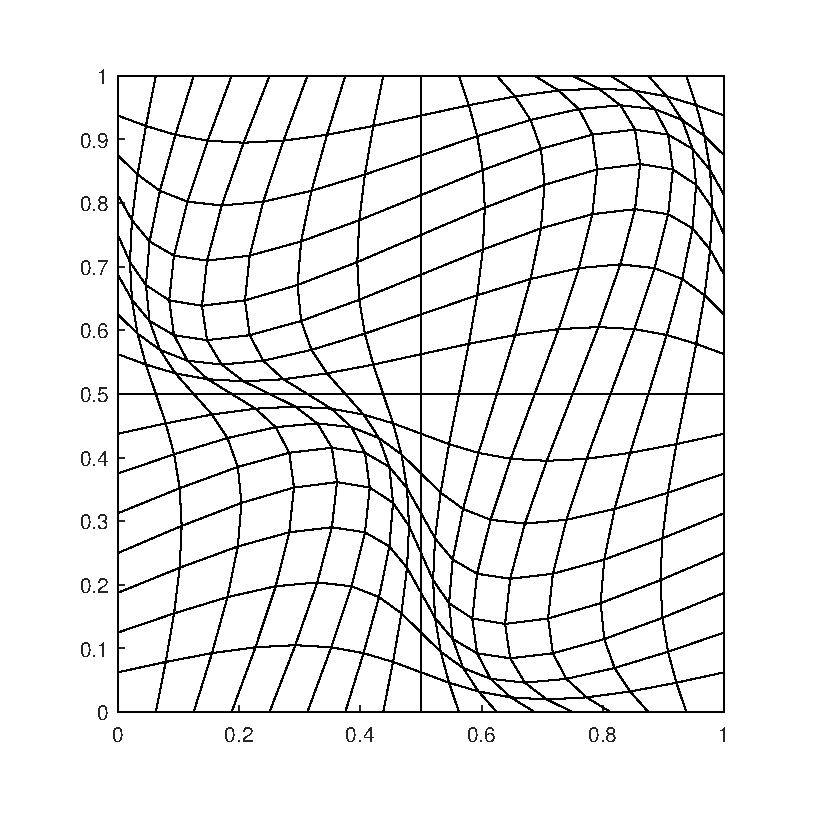
\includegraphics[width=0.3\linewidth]{pics/m6.eps}}
\caption{Types of meshes used in numerical experiments}
\label{fig:mesh}
\end{figure}

\begin{table}[h]
\centering
\begin{tabular}{ccccccc}
\hline
 & mesh (a) & mesh (b) & mesh (c) & mesh (d) & mesh (e) & mesh (f) \\
\hline
$L^2$ (EBS-1) & 3.52e-16 & 4.73e-16 & 3.72e-15 & 2.24e-15 & 9.28e-16 & 5.61e-16 \\
$L^\infty$ (EBS-1) & 6.80e-16 & 9.06e-16 & 1.36e-14 & 7.28e-15 & 1.51e-15 & 1.35e-15 \\
$L^2$ (EBS-2) & 1.74e-15 & 7.58e-16 & 1.97e-15 & 2.12e-15 & 5.28e-16 & 1.19e-15 \\
$L^\infty$ (EBS-2) & 3.02e-15 & 1.21e-15 & 5.68e-15 & 4.61e-15 & 1.21e-15 & 2.24e-15 \\
\hline
\end{tabular}
\caption{Errors of two edge centered schemes for linear solution on different meshes.}
\label{tab:linear}
\end{table}

\subsection{Unstructured meshes}

Consider the problem on $\Omega = [0,1]^2$ with constant anisotropic diffusion tensor and the exact solution given as follows:
\begin{align*}
\Lambda(x) =
\left(
\begin{matrix}
1.5 & 0.5 \\
0.5 & 1.5
\end{matrix}
\right),
\qquad
u(x,y) = \sin((x-1) \, (y-1)) - (x-1)^3 \, (y-1)^2.
\end{align*}
The locally refined mesh and the random polygonal mesh shown in \cref{fig:mesh} are used here. On the locally refined mesh, the error of EBS-1 is $E_2 = 0.99 \times 10^{-3}, E_\infty = 1.42 \times 10^{-3}$, and the error of EBS-2 is $E_2 = 1.66 \times 10^{-3}, E_\infty = 2.16 \times 10^{-3}$. On the random polygonal mesh, the error of EBS-1 is $E_2 = 4.62 \times 10^{-3}, E_\infty = 7.02 \times 10^{-3}$, and the error of EBS-2 is $E_2 = 5.37 \times 10^{-3}, E_\infty = 9.37 \times 10^{-3}$.
The numerical solution $u$ and the error function $u - u_{\text{exact}}$ of both schemes on corresponding meshes are shown in \cref{fig:solution}. 
One can see that edge centered schemes can handle the unstructured mesh well and achieve small error.

\begin{figure}[h]
\centering
\subfloat[solution of EBS-1]{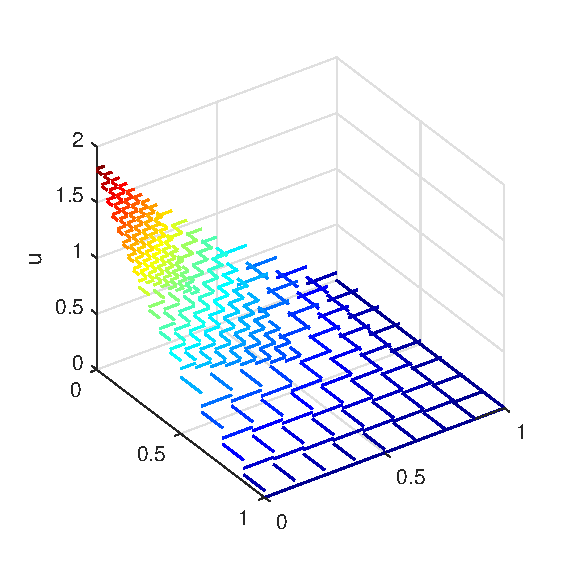
\includegraphics[width=0.22\linewidth]{pics/m1s1u.eps}}
\subfloat[error of EBS-1]{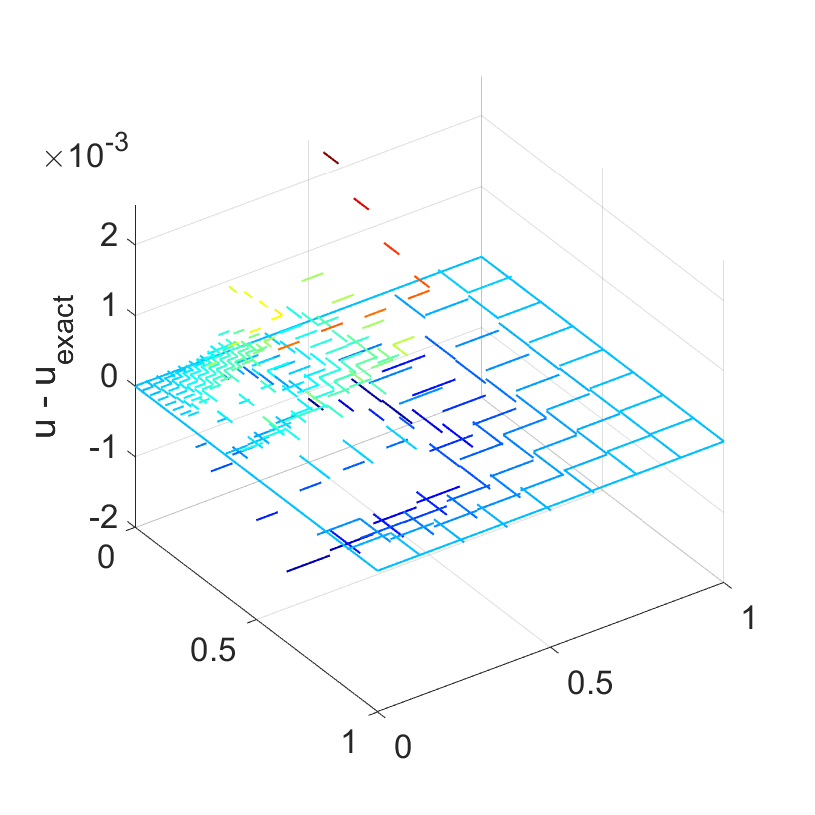
\includegraphics[width=0.22\linewidth]{pics/m1s1err.eps}}
\subfloat[solution of EBS-2]{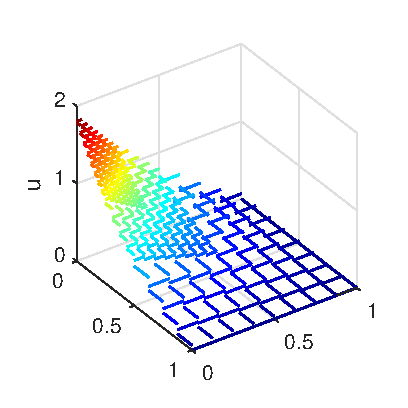
\includegraphics[width=0.22\linewidth]{pics/m1s2u.eps}}
\subfloat[error of EBS-2]{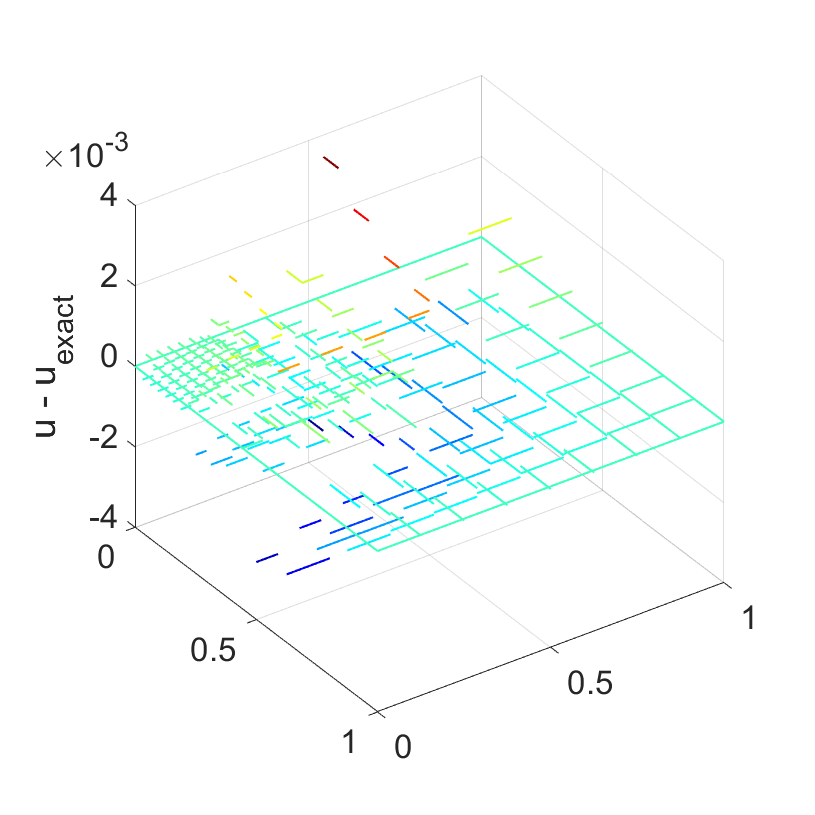
\includegraphics[width=0.22\linewidth]{pics/m1s2err.eps}} \\
\subfloat[solution of EBS-1]{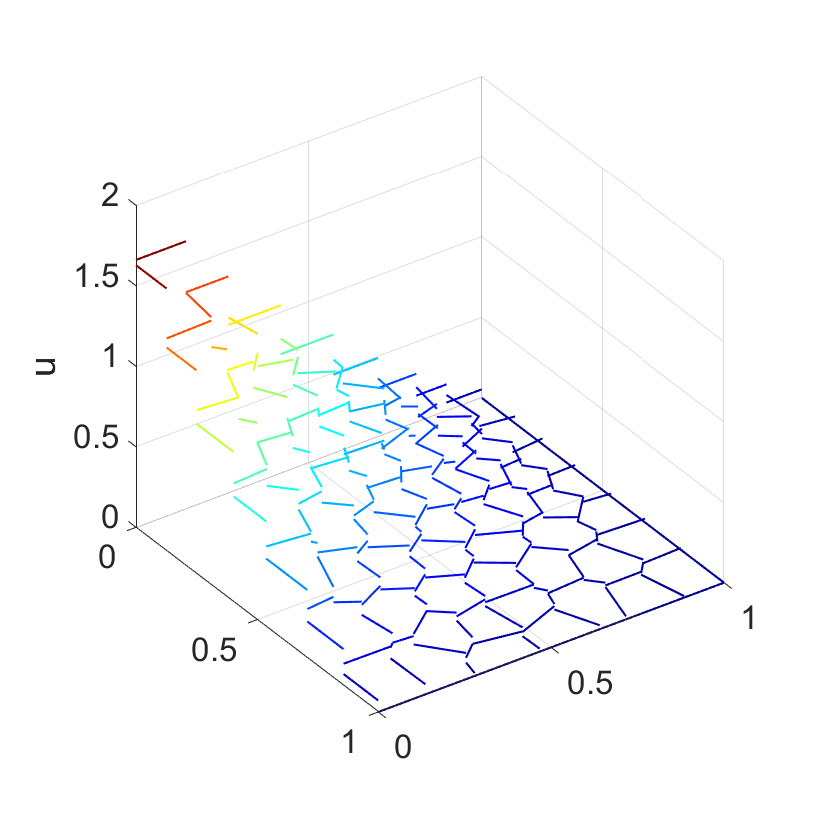
\includegraphics[width=0.22\linewidth]{pics/m2s1u.eps}}
\subfloat[error of EBS-1]{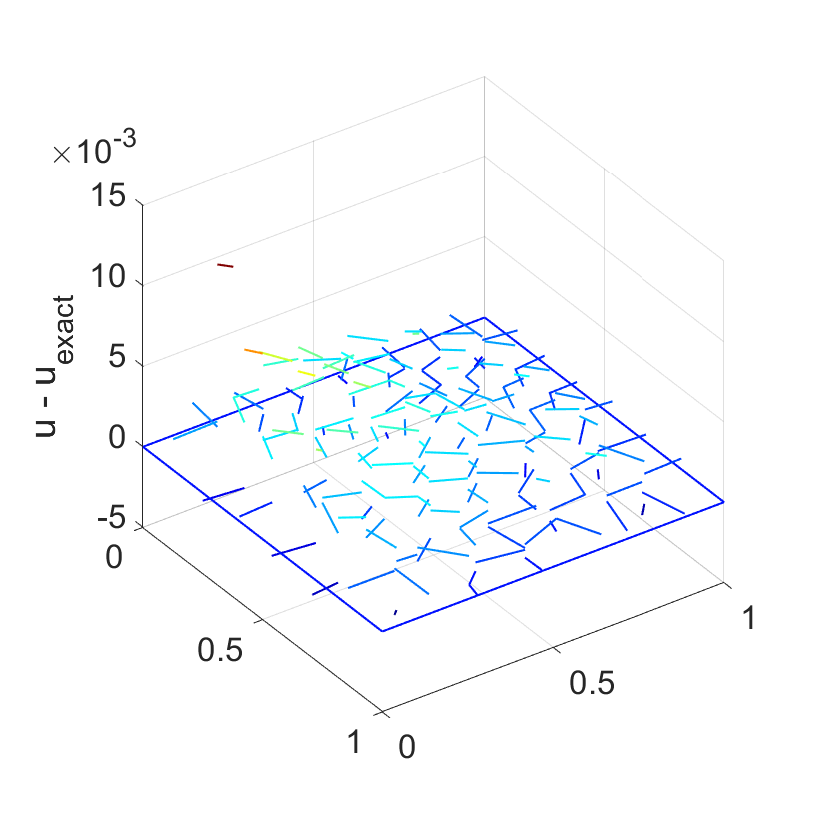
\includegraphics[width=0.22\linewidth]{pics/m2s1err.eps}}
\subfloat[solution of EBS-2]{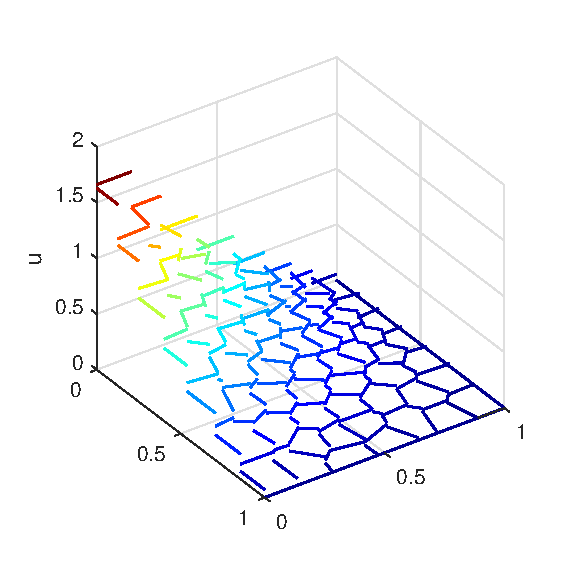
\includegraphics[width=0.22\linewidth]{pics/m2s2u.eps}}
\subfloat[error of EBS-2]{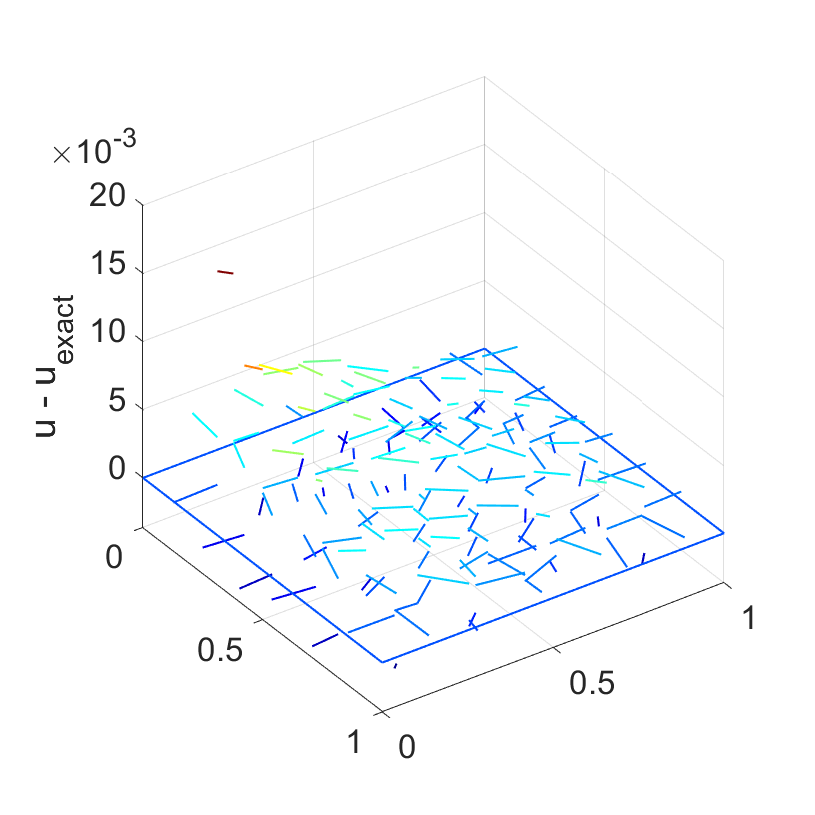
\includegraphics[width=0.22\linewidth]{pics/m2s2err.eps}}
\caption{Numerical solutions and error functions of two edge centered schemes on two types of meshes}
\label{fig:solution}
\end{figure}

\subsection{Accuracy of edge centered schemes}

To test the accuracy of edge centered schemes on distorted meshes, we consider a simple problem with diffusion tensor and exact solution given as follows:
\begin{align*}
\Lambda(x) =
\left(
\begin{matrix}
1.5 & 0.5 \\
0.5 & 1.5
\end{matrix}
\right),
\qquad
u(x,y) = 16 \, x \, (1-x) \, y \, (1-y).
\end{align*}
A family of skewed quadrilateral meshes are used. The distortion of meshes is the mean difficulty in this example. The results are presented in \cref{tab:skewed-2} and \cref{tab:skewed-inf}.
On such skewed meshes, NPS cannot attain optimal order because of the loss of precision in interpolation step, but EBS can attain optimal convergence order.

\begin{table}[h]
\centering
\begin{tabular}{cccccccccc}
\hline
\multirow{2}*{mesh size} & \multicolumn{3}{c}{NPS} & \multicolumn{3}{c}{EBS-1} & \multicolumn{3}{c}{EBS-2} \\
\cmidrule(r){2-4} \cmidrule(r){5-7} \cmidrule(r){8-10}
& DOF & $E_2$ & order & DOF & $E_2$ & order & DOF & $E_2$ & order \\
\hline
$17 \times 17$ & 289 & 3.24e-01 & * & 612 & 2.21e-02 & * & 612 & 2.18e-02 & * \\
$34 \times 34$ & 1156 & 2.70e-01 & 0.26 & 2380 & 5.64e-03 & 2.01 & 2380 & 5.57e-03 & 2.01 \\
$51 \times 51$ & 2601 & 2.31e-01 & 0.39 & 5304 & 2.51e-03 & 2.01 & 5304 & 2.48e-03 & 2.01 \\
$68 \times 68$ & 4624 & 2.00e-01 & 0.50 & 9384 & 1.42e-03 & 2.01 & 9384 & 1.40e-03 & 2.01 \\
$85 \times 85$ & 7225 & 1.77e-01 & 0.55 & 14620 & 9.07e-04 & 2.01 & 14620 & 8.96e-04 & 2.01 \\
$102 \times 102$ & 10404 & 1.58e-01 & 0.61 & 21012 & 6.30e-04 & 2.01 & 21012 & 6.22e-04 & 2.01 \\
\hline
\end{tabular}
\caption{$L^2$ relative error and convergence rate of different schemes on skewed quadrilateral meshes}
\label{tab:skewed-2}
\end{table}

\begin{table}[h]
\centering
\begin{tabular}{cccccccccc}
\hline
\multirow{2}*{mesh size} & \multicolumn{3}{c}{NPS} & \multicolumn{3}{c}{EBS-1} & \multicolumn{3}{c}{EBS-2} \\
\cmidrule(r){2-4} \cmidrule(r){5-7} \cmidrule(r){8-10}
& DOF & $E_\infty$ & order & DOF & $E_\infty$ & order & DOF & $E_\infty$ & order \\
\hline
$17 \times 17$ & 289 & 4.33e-01 & * & 612 & 5.80e-02 & * & 612 & 5.43e-02 & * \\
$34 \times 34$ & 1156 & 3.73e-01 & 0.22 & 2380 & 1.49e-02 & 2.00 & 2380 & 1.41e-02 & 1.98 \\
$51 \times 51$ & 2601 & 3.26e-01 & 0.33 & 5304 & 6.64e-03 & 2.02 & 5304 & 6.32e-03 & 2.01 \\
$68 \times 68$ & 4624 & 2.86e-01 & 0.45 & 9384 & 3.73e-03 & 2.02 & 9384 & 3.56e-03 & 2.01 \\
$85 \times 85$ & 7225 & 2.56e-01 & 0.51 & 14620 & 2.39e-03 & 2.01 & 14620 & 2.28e-03 & 2.01 \\
$102 \times 102$ & 10404 & 2.31e-01 & 0.56 & 21012 & 1.66e-03 & 2.01 & 21012 & 1.58e-03 & 2.01 \\
\hline
\end{tabular}
\caption{$L^\infty$ relative error and convergence rate of different schemes on skewed quadrilateral meshes}
\label{tab:skewed-inf}
\end{table}

\subsection{Anisotropic diffusion problems}

In practical applications, we often encounter the problems with distorted meshes and anisotropy. To test the accuracy of schemes for anisotropic problems, we consider
\begin{align*}
\Lambda(x) =
\left(
\begin{matrix}
1 & 0 \\
0 & \delta
\end{matrix}
\right),
\qquad
u(x,y) = \sin(2 \pi x) \, \exp(-\frac{2 \pi}{\sqrt{\delta}} y).
\end{align*}We take $\delta = 10^5$ then the problem has strong anisotropy. A sequence of Kershaw meshes are used. Kershaw mesh is recognized as challenging because of the distortion. The results are shown in \cref{tab:anis-2} and \cref{tab:anis-inf}. Edge centered schemes works well in this experiment.

\begin{table}[h]
\centering
\begin{tabular}{cccccccccc}
\hline
\multirow{2}*{mesh size} & \multicolumn{3}{c}{NPS} & \multicolumn{3}{c}{EBS-1} & \multicolumn{3}{c}{EBS-2} \\
\cmidrule(r){2-4} \cmidrule(r){5-7} \cmidrule(r){8-10}
& DOF & $E_2$ & order & DOF & $E_2$ & order & DOF & $E_2$ & order \\
\hline
$4 \times 4$ & 16 & 2.80e-01 & * & 40 & 2.93e-01 & * & 40 & 9.50e-02 & * \\
$8 \times 8$ & 64 & 8.13e-02 & 1.78 & 144 & 5.82e-02 & 2.52 & 144 & 2.78e-02 & 1.92 \\
$16 \times 16$ & 256 & 2.37e-02 & 1.78 & 544 & 1.39e-02 & 2.16 & 544 & 5.07e-03 & 2.56 \\
$32 \times 32$ & 1024 & 7.45e-03 & 1.67 & 2112 & 3.42e-03 & 2.06 & 2112 & 1.17e-03 & 2.16 \\
$64 \times 64$ & 4096 & 2.48e-03 & 1.58 & 8320 & 8.53e-04 & 2.03 & 8320 & 2.86e-04 & 2.05 \\
$128 \times 128$ & 16384 & 8.48e-04 & 1.55 & 33024 & 2.13e-04 & 2.01 & 33024 & 7.11e-05 & 2.02 \\
\hline
\end{tabular}
\caption{$L^2$ relative error and convergence rate of different schemes for the anistropic problem}
\label{tab:anis-2}
\end{table}

\begin{table}[h]
\centering
\begin{tabular}{cccccccccc}
\hline
\multirow{2}*{mesh size} & \multicolumn{3}{c}{NPS} & \multicolumn{3}{c}{EBS-1} & \multicolumn{3}{c}{EBS-2} \\
\cmidrule(r){2-4} \cmidrule(r){5-7} \cmidrule(r){8-10}
& DOF & $E_\infty$ & order & DOF & $E_\infty$ & order & DOF & $E_\infty$ & order \\
\hline
$4 \times 4$ & 16 & 3.53e-01 & * & 40 & 4.16e-01 & * & 40 & 2.89e-01 & * \\
$8 \times 8$ & 64 & 1.24e-01 & 1.51 & 144 & 8.29e-02 & 2.52 & 144 & 9.54e-02 & 1.73 \\
$16 \times 16$ & 256 & 6.54e-02 & 0.92 & 544 & 1.99e-02 & 2.15 & 544 & 1.96e-02 & 2.38 \\
$32 \times 32$ & 1024 & 3.06e-02 & 1.10 & 2112 & 4.88e-03 & 2.07 & 2112 & 4.19e-03 & 2.27 \\
$64 \times 64$ & 4096 & 1.44e-02 & 1.09 & 8320 & 1.21e-03 & 2.03 & 8320 & 9.62e-04 & 2.14 \\
$128 \times 128$ & 16384 & 6.85e-03 & 1.07 & 33024 & 3.03e-04 & 2.01 & 33024 & 2.31e-04 & 2.07 \\
\hline
\end{tabular}
\caption{$L^\infty$ relative error and convergence rate of different schemes for the anistropic problem}
\label{tab:anis-inf}
\end{table}

\subsection{Heterogeneous diffusion problems}

Heterogeneous is represented by the discontinuity of diffusion tensor  in the model, which is very common in practical calculations. To test the ability of schemes for handling heterogeneous problems, we divide the domain $\Omega = [0,1]^2$ into four parts, the diffusion tensor and the solution on each part is chosen as
\begin{align*}
\Lambda =
\left(
\begin{matrix}
a_1 & 0 \\
0 & a_2
\end{matrix}
\right),
\qquad
u(x,y) = \alpha \, \sin(2 \pi x) \, \sin(2 \pi y),
\end{align*}
where
\begin{equation*}
\left\{
\begin{array}{llllll}
a_1 = 10, & a_2 = 0.01, & \alpha = 0.1 & \text{for} & 0 < x \leq 0.5, & 0 < y \leq 0.5, \\
a_1 = 0.1, & a_2 = 100, & \alpha = 10 & \text{for} & 0.5 < x < 1, & 0 < y \leq 0.5, \\
a_1 = 100, & a_2 = 0.1, & \alpha = 0.01 & \text{for} & 0 < x \leq 0.5, & 0.5 < y < 1, \\
a_1 = 0.01, & a_2 = 10, & \alpha = 100 & \text{for} & 0.5 < x < 1, & 0.5 < y < 1. \\
\end{array}
\right.
\end{equation*}
A sequence of triangular meshes with type shown in \cref{fig:mesh}(e) are used. The results are shown in \cref{tab:anis-2} and \cref{tab:anis-inf}. One can see that both edge centered schemes are same on triangular meshes. Though the relative error of edge centered schemes are big, edge centered schemes presents the optimal order.

\begin{table}[h]
\centering
\begin{tabular}{cccccccccc}
\hline
\multirow{2}*{mesh size} & \multicolumn{3}{c}{NPS} & \multicolumn{3}{c}{EBS-1} & \multicolumn{3}{c}{EBS-2} \\
\cmidrule(r){2-4} \cmidrule(r){5-7} \cmidrule(r){8-10}
& DOF & $E_2$ & order & DOF & $E_2$ & order & DOF & $E_2$ & order \\
\hline
$2 \times 2$ & 56 & 4.44e-01 & * & 92 & 9.33e+01 & * & 92 & 9.33e+01 & * \\
$4 \times 4$ & 224 & 1.94e-01 & 1.19 & 352 & 1.63e+01 & 2.60 & 352 & 1.63e+01 & 2.60 \\
$8 \times 8$ & 896 & 8.97e-02 & 1.11 & 1376 & 3.68e+00 & 2.18 & 1376 & 3.68e+00 & 2.18 \\
$16 \times 16$ & 3584 & 4.39e-02 & 1.03 & 5440 & 7.45e-01 & 2.32 & 5440 & 7.45e-01 & 2.32 \\
$32 \times 32$ & 14336 & 2.13e-02 & 1.04 & 21632 & 1.59e-01 & 2.24 & 21632 & 1.59e-01 & 2.24 \\
$64 \times 64$ & 57344 & 9.71e-03 & 1.14 & 86272 & 3.73e-02 & 2.09 & 86272 & 3.73e-02 & 2.09 \\
\hline
\end{tabular}
\caption{$L^2$ relative error and convergence rate of different schemes for the heterogeneous problem}
\label{tab:hetero-2}
\end{table}

\begin{table}[]
\centering
\begin{tabular}{cccccccccc}
\hline
\multirow{2}*{mesh size} & \multicolumn{3}{c}{NPS} & \multicolumn{3}{c}{EBS-1} & \multicolumn{3}{c}{EBS-2} \\
\cmidrule(r){2-4} \cmidrule(r){5-7} \cmidrule(r){8-10}
& DOF & $E_\infty$ & order & DOF & $E_\infty$ & order & DOF & $E_\infty$ & order \\
\hline
$2 \times 2$ & 56 & 4.10e-01 & * & 92 & 7.67e+01 & * & 92 & 7.67e+01 & * \\
$4 \times 4$ & 224 & 2.81e-01 & 0.54 & 352 & 2.44e+01 & 1.71 & 352 & 2.44e+01 & 1.71 \\
$8 \times 8$ & 896 & 1.64e-01 & 0.78 & 1376 & 5.67e+00 & 2.14 & 1376 & 5.67e+00 & 2.14 \\
$16 \times 16$ & 3584 & 8.90e-02 & 0.88 & 5440 & 1.22e+00 & 2.24 & 5440 & 1.22e+00 & 2.24 \\
$32 \times 32$ & 14336 & 5.20e-02 & 0.78 & 21632 & 2.94e-01 & 2.06 & 21632 & 2.94e-01 & 2.06 \\
$64 \times 64$ & 57344 & 3.20e-02 & 0.70 & 86272 & 7.26e-02 & 2.02 & 86272 & 7.26e-02 & 2.02 \\
\hline
\end{tabular}
\caption{$L^\infty$ relative error and convergence rate of different schemes for the heterogeneous problem}
\label{tab:hetero-inf}
\end{table}

\subsection{Robustness on Heterogeneous rotating anisotropy}

Finally, noting that we introduce a stabilization parameter $\gamma$ in EBS-2, we want to verify that scheme is robust under different $\gamma$. Here we choose the problem as
\begin{align*}
\Lambda(x,y) = 
\frac{1}{x^2 + y^2}
\left(
\begin{matrix}
\delta \, x^2 + y^2 & (\delta-1) \, x \, y \\
(\delta-1) \, x \, y  & x^2 + \delta \, y^2
\end{matrix}
\right),
\qquad
u(x,y) = sin(\pi \, x) \, \sin(\pi \, y).
\end{align*}
The parameter is chosen as $\delta = 10^{-3}$ here. A sequence of sin meshes are used.

This problem is universally considered as challenging \cite{???}. Here we test the problem using the schemes mentioned above under a wide range of parameter $\gamma$. The result is shown in \cref{fig:error}. From the figure on can see that NPS cannot attain optimal order, but both edge centered schemes under different parameters are all of second order. In this example, a small $\gamma$ will only make error increase, but makes no influence to the convergence order.

\begin{figure}[h]
\centering
\subfloat[$L^2$ error]{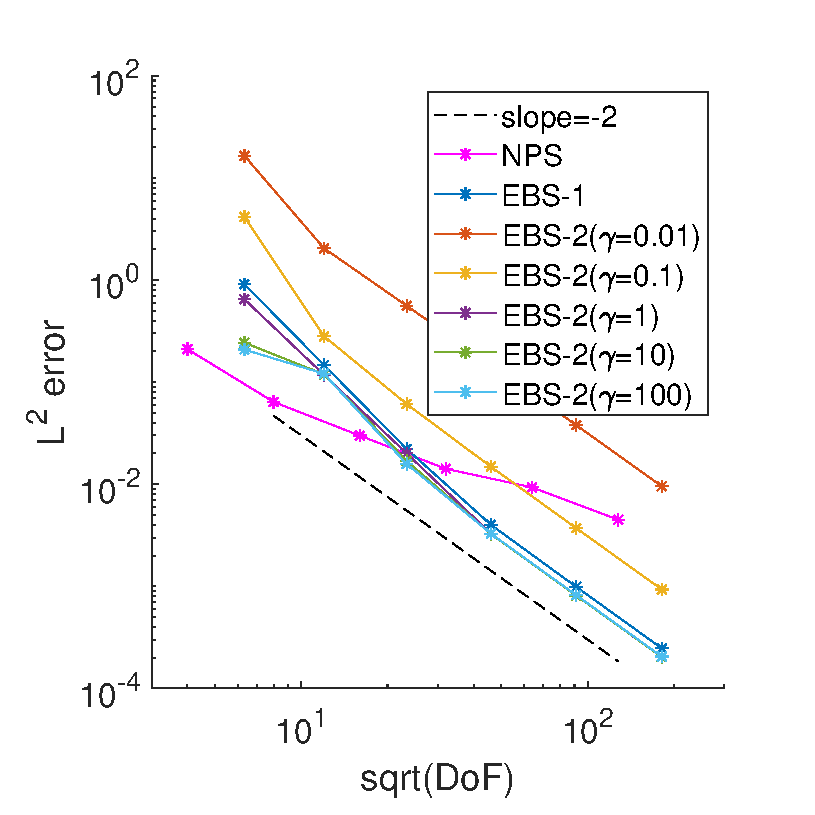
\includegraphics[width=0.33\linewidth]{pics/m6-2.eps}}
\subfloat[$L^\infty$ error]{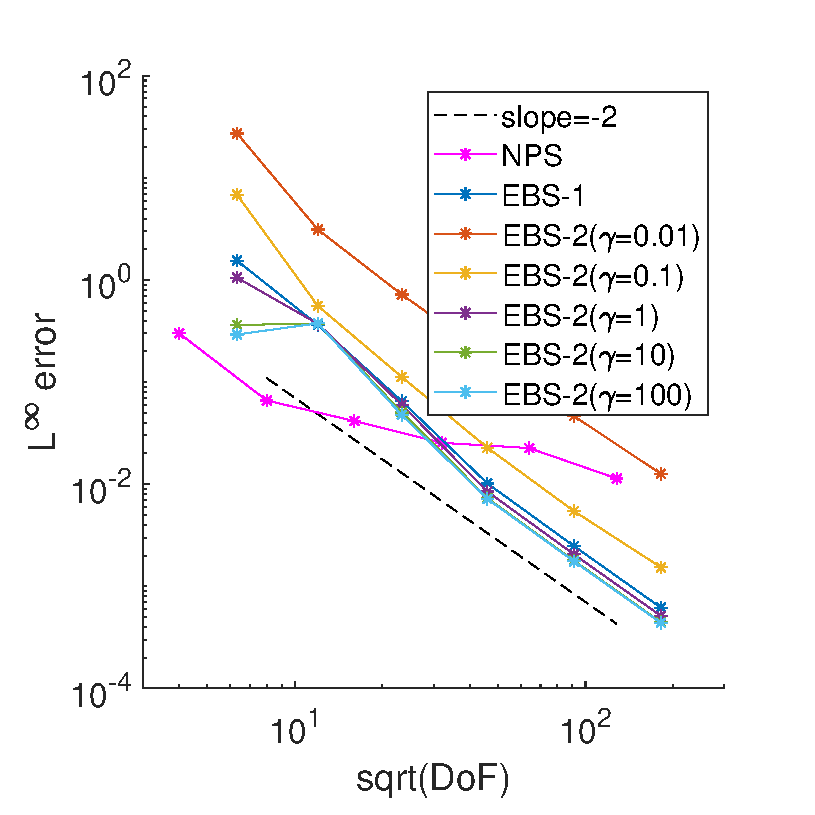
\includegraphics[width=0.33\linewidth]{pics/m6-inf.eps}}
\caption{$L^2$ and $L^\infty$ relative errors versus DoF for the schemes under different parameters.}
\label{fig:error}
\end{figure}

\section{Conclusion}\label{sec6}

In this article, we have presented a family of edge centered scheme (EBS-1 and EBS-2) for two-dimensional diffusion problems.
The schemes takes into account the general polygonal meshes and arbitrary heterogeneous anisotropic diffusion tensors.
The scheme EBS-2 is proved to be symmetric and coercive under general assumptions.
Many numerical tests using unstructured and severely distorted meshes and arbitrary (continuous or discontinuous) anisotropic diffusion tensors show the accuracy and robustness of the scheme.

The extension of the present scheme to 3D polyhedral grids is not so easy but still possible, which constitute the topics of a future work.
Further, constructing a edge centered scheme which satisfies discrete maximum principle is also our future work.

\section*{Acknowledgments}

This work was supported by nothing.

%%Vancouver style references.
\begin{thebibliography}{100}

\bibitem{Aavatsmark2002}
I. Aavatsmark, An introduction to multipoint flux approximations for quadrilateral grids, Comput. Geosci. 6 (2002) 405-432.


\bibitem{Aavatsmark1998}
I. Aavatsmark, T. Barkve, O. B$\Phi$e, T. Mannseth, Discretization on unstructured grids for inhomogeneous, anisotropic media. I. Derivation of the methods, SIAM J. Sci. Comput. 19 (1998) 1700-1716.

\bibitem{Aavatsmark2008}
I. Aavatsmark, G.T. Eigestad, B.T. Mallison and J. M. Nordbotten, A compact multipoint flux approximation method with improved robustness, Numer. Methods Partial. Differ. Eqs. 24 (2008) 1329-1360.

\bibitem{Agelas2010}
L. Agelas, D.A. Di Pietro, J. Droniou, The G method for heterogeneous anisotropic diffusion on general meshes, ESAIM: Math. Model. Numer. Anal. 44 (2010) 597-625.

\bibitem{Agelas-Eymard2009}
L. Agelas, R. Eymard, R. Herbin, A nine-point finite volume scheme for the simulation of diffusion in heterogeneous media, C.R. Acad. Sci. Paris, Ser. I 347 (2009) 673-676.

\bibitem{Andreianov2007}
B. Andreianov, F. Boyer, F. Hubert, Discrete duality finite volume schemes for Leray-Lions-type elliptic problems on general 2D meshes, Numer. Methods Partial Differ. Eqs. 23 (2007) 145-195.

\bibitem{Boyer2008}
F. Boyer, F. Hubert, Finite volume method for 2D linear and nonlinear elliptic problems with discontinuities, SIAM J. Numer. Anal. 46 (2008)
3032-3070.

\bibitem{Brezzi2005_1}
F. Brezzi, K. Lipnikov, . Shashkov, Convergence of the mimetic finite difference method for diffusion problems on polyhedral meshes, SIAM J. Numer. Anal. 43 (2005) 1872-1896.

\bibitem{Brezzi2005_2}
F. Brezzi, K. Lipnikov, V. Simoncini, A family of mimetic finite difference methods on polygonal and polyhedral meshes, Math. Models Methods Appl. Sci. 15 (2005) 1533-1551.

\bibitem{C-C-L-C}
T. {\color{black}de} M. Cavalcante, F.R.L. Contreras, P.R.M. Lyra, D.K.E. de Carvalho, A multipoint flux
approximation with diamond stencil finite volume scheme for the two-dimensional simulation of fluid flows in naturally fractured reservoirs using a hybrid-grid method, Int. J. Numer. Meth. Fluids. 92 (2020) 1322-1351.

\bibitem{C-L-S-C}
F.R.L. Contreras, P.R.M. Lyra, M.R.A. Souza, D.K.E. de Carvalho, A cell-centered multipoint flux approximation method with a diamond stencil coupled with a higher order finite volume method for the simulation of oil-water displacements in heterogeneous and anisotropic petroleum
reservoirs, Comput{\color{black}.} Fluids. 127 (2016) 1-16.


\bibitem{Y-J-P}
Y. Coudi\`{e}re, J.-P. Vila, P. Villedieu, Convergence rate of a finite volume scheme for
a {\color{black} two dimensional convection-diffusion} problem, ESAIM: Math. Model. Numer. Anal. 33
(1999) 493-516.



 {\color{black}
\bibitem{DANILOV2009}
A. Danilov, Y. Vassilevski, A monotone nonlinear finite volume method
for diffusion equations on conformal polyhedral meshes, Russ. J. Numer. Anal. Math. Model. 24 (2009), 207-227.}

\bibitem{Zhang-Ding2012}
N. Ding, Y. Zhang, D. Xiao, J. Wu, Z. Dai, L. Yin, Z. Gao,
S. Sun, C. Xue, C. Ning, X. Shu, J. Wang, Theoretical and numerical research of wire array Z-pinch and dynamic
hohlraum at IAPCM, Matter and Radiation at Extremes, 1(2016) 135-152.

\bibitem{Droniou2014}
J. Droniou, Finite volume schemes for diffusion equations: Introduction to and review of modern methods,  Math. Models Methods Appl. Sci. 24 (2014) 1575-1619.

\bibitem{Droniou2006}
J. Droniou, R. Eymard, A mixed finite volume scheme for anisotropic diffusion problems on any grid, Numer. Math. 105 (2006) 35-71.

\bibitem{Edwards-Zheng}
M.G. Edwards, Unstructured, control-volume distributed, full-tensor finite-volume
schemes with flow-based grids, Comput. Geosci. 6 (2002) 433-452.




\bibitem{Eymard2010}
R. Eymard, T. Gallouet, R. Herbin, Discretization of heterogeneous and anisotropic diffusion problems on general nonconforming meshes SUSHI: A scheme using stabilization and hybrid interfaces, IMA J. Numer. Anal. 30 (2010) 1009-1043.




\bibitem{Eymard-Herbin2012}
R. Eymard, R. Herbin, C. Guichard, Small-stencil 3D schemes for diffusive flows in porous media, Math. Model. Numer. Anal. 46 (2012) 265-290.

\bibitem{Z. Gao-J. Wu}
Z. Gao, J. Wu, A second-order positivity-preserving finite volume scheme for diffusion equations on general meshes,  SIAM J. Sci. Comput.  37 (2015) {\color{black}A420-A438}.

\bibitem{gao-wu}
Z. Gao, J. Wu, A linearity-preserving cell-centered scheme for the heterogeneous
and anisotropic diffusion equations on general meshes, Int. J. Numer. Meth. Fluids 67 (2011) 2157-2183.


\bibitem{Gao-Wu2013}
Z. Gao, J. Wu, A small stencil and extremum-preserving scheme for anisotropic diffusion problems on arbitrary 2D and 3D meshes, J. Comput. Phys. 250 (2013) 308-331.



\bibitem{Herbin}
R. Herbin,   F. Hubert, Benchmark on discretization schemes for anisotropic diffusion problems on
general grids,  {\color{black}in: R. Eymard, J. -M. H\'erard}, (Eds.),
Finite Volumes for Complex Applications V, {\color{black} Wiley, (2008) 659-692}.

\bibitem{Hermeline2000}
F. Hermeline, A finite volume method for the approximation of diffusion operators on distorted meshes, J. Comput. Phys. 160 (2000) 481-499.



\bibitem{li1980}
D. Li, H. Shui, M. Tang, On the finite difference scheme of two-dimensional parabolic equation in a non-rectangular mesh, J. Numer. Methods
Comput. Appl. 1 (1980) 217-224 (in Chinese).

\bibitem{Lipnikov2007}
 K. Lipnikov, M. Shashkov, D. Svyatskiy, Y. Vassilevski, Monotone finite volume schemes for diffusion equations on unstructured triangular and shape regular polygonal meshes, J. Comput. Phys. 227 (2007) 492-512.










\bibitem{Lipnikov2009}
K. Lipnikov, D. Svyatskiy, Y. Vassilevski, Interpolation-free monotone finite volume method for diffusion equations on polygonal meshes, J. Comput.
Phys. 228 (2009)  703-716.

\bibitem{Lipnikov-Svyatskiy2010}
K. Lipnikov, D. Svyatskiy, Y. Vassilevski, A monotone finite volume method for advection-diffusion equations on unstructured polygonal meshes, J. Comput. Phys. 229 (2010) 4017-4032.

\bibitem{Lipnikov2012}
K. Lipnikov, D. Svyatskiy, Yu. Vassilevski, Minimal stencil finite volume scheme with the discrete maximum principle, Russ. J. Numer. Anal. Math. Model. 27 (4) (2012) 369-386.

\bibitem{Lipnikov-Svyatskiy2013}
K. Lipnikov, D. Svyatskiy, Y. Vassilevski, Anderson acceleration for nonlinear finite volume scheme for advection-diffusion problems, SIAM J. Sci. Comput. 35 (2013) A1120-A1136.
%
\bibitem{G-M}
 G. Manzini, M. Putti, Mesh locking effects in the finite volume solution of 2-D anisotropic diffusion equations, J. Comput. Phys. 220 (2007) 751-771.


\bibitem{zhu2021}
W. Mao, Y. Zhu, M. Ye, X. Zhang, J. Wu, J. Yang,
A new quasi-3-D model with a dual iterative coupling scheme for simulating unsaturated-saturated water flow and solute transport at a regional scale,
J. Hydrol. 602 (2021) 126780.


\bibitem{MiaoWu2022}
S. Miao, J. Wu, A nonlinear correction scheme for the heterogeneous and anisotropic diffusion problems on polygonal meshes, J. Comput. Phys. 448 (2022) 110729.


\bibitem{MiaoYao2021}
S. Miao, Y. Yao, G. Lv, An efficient parallel iteration algorithm for nonlinear diffusion equations with time extrapolation techniques and the Jacobi explicit scheme, J. Comput. Phys. 441 (2021) 110435.

\bibitem{Morel1998}
J. Morel, R. Roberts, M. Shashkov, A local support-operators diffusion discretization scheme for quadrilateral r-z meshes, J. Comput. Phys. 144 (1998) 17-51.

\bibitem{Mousseau2003}
V. Mousseau, D. Knoll, New physics-based preconditioning of implicit methods for non-equilibrium radiation diffusion, J. Comput. Phys. 190 (2003) 42-51.


\bibitem{Potier}
C. Le Potier,  A second order in space combination of methods verifying a maximum principle for the discretization of diffusion operators, C. R. Math. Acad, Sci. Paris.  {\color{black}358} (2020) 89-95.

\bibitem{Potier CL}
 C. Le Potier, Sch{\color{black}\'e}ma volumes finis monotone pour des op{\color{black}\'e}rateurs de diffusion fortement anisotropes sur des maillages de triangle{\color{black}s} non structur{\color{black}\'e}s, {\color{black}C. R. Acad. Sci. Paris, Ser. I} 341 (2005) 787-792.



\bibitem{Schneider2017}
M. Schneider, L. Ag{\color{black}\'e}las, G. Ench{\color{black}\'e}ry, B. Flemisch, Convergence of nonlinear finite volume
schemes for heterogeneous anisotropic diffusion on general meshes, J. Comput. Phys. 351 (2017) 80-107.

{\color{black}
\bibitem{Schneider2018}
M. Schneider, D. Gl\"{a}ser, B. Flemisch, R. Helmig, Comparison of finite-volume schemes for diffusion problems, Oil Gas Sci. Technol. - Rev. IFP Energ. Nouv. 73 (2018), 82.}


\bibitem{Shashkov1995}
M. Shashkov, S. Steinberg, Support-operator finite-difference algorithms for general elliptic problems, J. Comput. Phys. 118 (1995) 131-151.



\bibitem{su2018}
S. Su, Q. Dong, J. Wu, A decoupled and positivity-preserving discrete duality finite volume scheme for anisotropic diffusion problems on general polygonal meshes, J. Comput. Phys. 372(2018) 773-798.



\bibitem{sunwuzhang2013}
W. Sun, J. Wu, X. Zhang, A family of linearity-preserving schemes for anisotropic diffusion problems on arbitrary polyhedral grids, Comput. Methods Appl. Mech. Eng. 267 (2013) 418-433.



\bibitem{Terekhov2017}
K.M. Terekhov, B.T. Mallison, H.A. Tchelepi, Cell-centered nonlinear finite-volume methods for the heterogeneous anisotropic diffusion problem, J. Comput. Phys. 330 (2017) 245-267.

{\color{black}
\bibitem{Vassilevski2020}
Y. Vassilevski, K. Terekhov, K. Nikitin, I. Kapyrin, Parallel Finite Volume Computation on General Meshes,  Springer, Switzerland, 2020.}



\bibitem{V-D-D2013}
D. Vidovi{\color{black}\'c}, M. Dotli{\color{black}\'c}, M. Dimki{\color{black}\'c}, M. Pu{\color{black}$\check{\hbox{s}}$}i{\color{black}\'c}, B. Pokorni, Convex combinations for diffusion schemes, J. Comput. Phys. 246 (2013) 11-27.

\bibitem{V-D-D2011}
D. Vidovi{\color{black}\'c}, M. Dotli{\color{black}\'c},  M. Pu{\color{black}$\check{\hbox{s}}$}i{\color{black}\'c},  Accelerated non-linear finite volume method for diffusion, J. Comput. Phys. 230 (2011) 2722-2735.




\bibitem{Wu-Dai-Gao-Yuan}
J. Wu, Z. Dai, Z. Gao, G. Yuan, Linearity preserving nine-point schemes for diffusion equation on distorted quadrilateral meshes, J. Comput.
Phys. 229 (2010) 3382-3401.


\bibitem{J. Wu-Z. Gao}
J. Wu, Z. Gao, Interpolation-based second-order monotone finite volume schemes for
anisotropic diffusion equations on general grids, J. Comput. Phys. 275 (2014), 569-588.


\bibitem{wugaodai2012}
J. Wu, Z. Gao, Z. Dai, A stabilized linearity-preserving scheme for the heterogeneous and anisotropic diffusion problems on polygonal meshes, J. Comput. Phys. 231 (2012) 7152-7169.

\bibitem{Wu-Gao-Dai}
J. Wu,  Z. Gao, Z. Dai, A vertex-centered linearity-preserving discretization of diffusion problems on polygonal meshes,  Int. J. Numer. Meth. Fluids 81 (2016) 131-150.


\bibitem{Xie-Xu2021}
H. Xie, X. Xu, C. Zhai, H. Yong, A positivity-preserving finite volume scheme with least square interpolation for 3D anisotropic diffusion equation, J. Sci. Comput. 89 (2021) 53.

\bibitem{yuan2008}
G. Yuan, Z. Sheng, Monotone finite volume schemes for diffusion equations on polygonal meshes, J. Comput. Phys. 227 (2008) 6288-6312.


\bibitem{WZhang2020}
W. Zhang, M. Kobaisi, Cell-centered nonlinear finite-volume methods with improved robustness, SPE J. 25 (2020) 288-309.



\end{thebibliography}

\end{document}